\begin{figure*}[t]
	\centering
	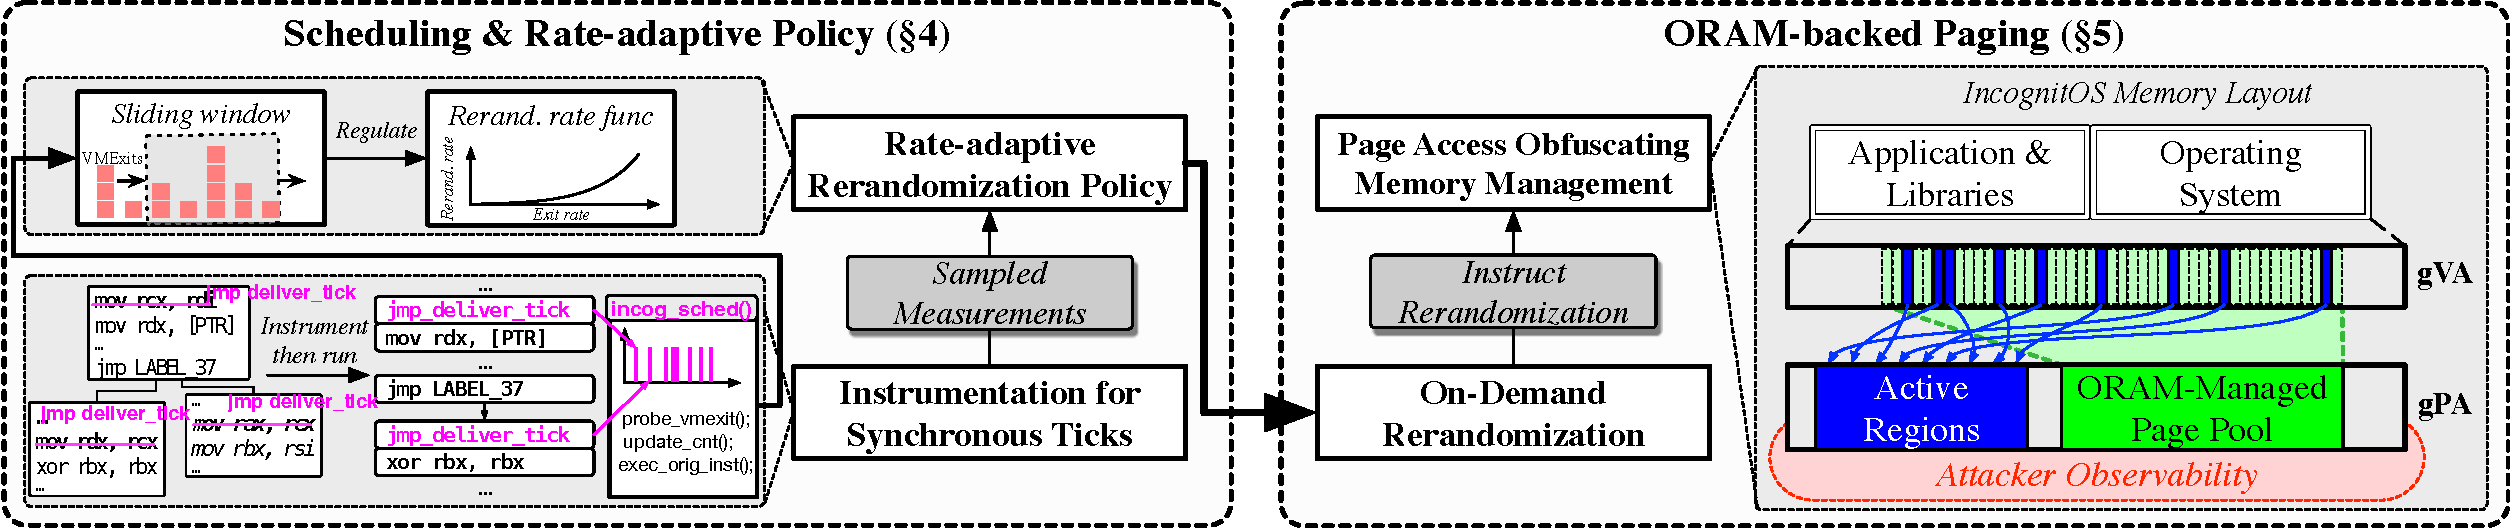
\includegraphics[width=0.99\textwidth]{figures/incognitos/incognitos-overview-v4.pdf}
	\caption{Overview of \thename}
	\label{fig:overview}
\end{figure*}

\section{\thename Overview}
\label{sec:overview}

\thename (\autoref{fig:overview}) is a unikernel design that targets AMD SEV-SNP for practical and transparent system-level defense against \gls{cvm} side-channel attacks.
It proposes a novel \emph{rate-adaptive obfuscation} scheme that allows relaxing the rerandomization rate during normal execution, as \thename can sense the symptoms of attacks and reactively increase the rate.




\subsection{Kernel subsystems}
As shown in \autoref{fig:overview}, \thename retrofits the following kernel subsystems to enforce its rate-adaptive obfuscation scheme.

\hdr{Scheduling subsystem}
% Our scheduling subsystem 
\thename's scheduling subsystem (\cref{sec:scheduling}) constructs a sampling system that can accurately determine the current VMExit rate.
Using the measured frequency of VMExit, the subsystem establishes a high-level \emph{rerandomization policy} to regulate the system's obfuscation.
To this end, \thename's scheduler implements a trustworthy self-invocation mechanism independent of the untrustworthy timer interrupts.
Our design decision was to implement so-called \emph{synchronous} ticks inserted throughout the user program and kernel to invoke the scheduler.
% On top of this self-sovereign scheduling mechanism, \thename establish a sampling system that can accurately determine the current VMExit rate.
% On the measured rate of VMExit, \freqvmexit, it constructs high-level \emph{rerandomization policies} to regulate the system's obfuscation strategy.
% However, \thename must stay transparent to the userspace (\reqtransparent)
% With a robust VMExit frequency measurement, a high-levvel rerandomization policy can be constructed to regulate the defense according to the sampled rates (\reqrobustpolicy).


\hdr{Paging subsystem}
The paging subsystem (\cref{sec:paging}) takes advantage of the direct access to the hardware MMU now available to \glspl{cvm} to implement a page rerandomization scheme.
It integrates an ORAM scheme into the OS page tables to perform secure page-ins and page-outs.
It performs on-demand rerandomization at a frequency regulated by the scheduler.
\thename paging allows the \gls{cvm} to enjoy full freedom using the \gls{gva} space, as \thename's rerandomization is achieved transparently in the OS-level.
% By only reshaping the \gls{gpa}, while keeping the \gls{gva} intact, 



\subsection{System requirements}
\thename's scheduling and paging subsystem must achieve functional design requirements (\reqsovereign-\reqfullsystem) while respecting the userspace by maintaining transparency (\reqtransparent).
\vspace{0.1em}

% \newcommand{\reqtrans}[0]{\textbf{R1}\xspace}
% \newcommand{\reqsched}[0]{\textbf{R2}\xspace}
% \newcommand{\reqsampling}[0]{\textbf{R3}\xspace}
% \newcommand{\reqfullsystem}[0]{\textbf{R4}\xspace}




\hdr{R1: Transparent Obfuscation} As an operating system, \thename's obfuscated execution must be transparent to the user programs that it hosts.
It must not require porting or even recompilation of the user programs.
This requirement has an impact on many design decisions made in \thename.
For instance, while \thename's synchronous ticks and VMExit sampling system resemble methods used in a previous work~\cite{oleksenko2018varys}, it leverages static binary instrumentation to support unmodified binaries.


\hdr{R2: Self-sovereign scheduling} \thename must implement a self-sovereign way of scheduling critical tasks independent of the timer interrupts the hypervisor delivers due to untrustworthy virtualized interrupts (\cref{sec:background:interrupts}).
At each scheduling \emph{tick}, \thename can carry out self-defensive operations such as measuring the current VMExit rate and rerandomizing CVM memory as necessary.


\hdr{R3: Robust VMExit rate sampling and policy} \thename's scheduling must be equipped with a robust VMExit rate sampling system.
Accurately and continuously measuring the VMExit rate is not a trivial task.
For instance, what is the system's necessary sampling rate for accurately sampling the VMExit frequency range of the attacks?
This robust sampling allows us to build a high-level policy that moderates the rerandomization rate.

\hdr{R4: Full-system memory rerandomization}
\thename's rerandomization of CVM memory must be transparent to userspace and, at the same time, must also include the kernel components.
Notably, we found that rerandomizing the locations of the page tables themselves is indispensable to avoid leaking \thename's memory layout.



\subsection{Embracing unikernel design }
\label{sec:overview:unikernel}

% \limcomm{I think this paragraph should explain why unikernel is a good choice, by refering each R1,R2,R3 or R4}{*}
\thename makes a case for unikernels as a basis for efficient transparent (\reqtransparent) and full-system (\reqfullsystem) obfuscation of \glspl{cvm}.
% \thename is a fork of the Unikfraft unikernel~\cite{unikraft} (v0.15.0) with its own implementation of AMD SEV-SNP~\cite{kaplanamd} support and a new I/O software stack that interoperates with SEV-compatible \texttt{virtio} drivers.
The unikernel-based approach brings the following unique design leverages.
% \limcomm{Remove?}{
% \thename proposes a unikernel-based full-system obfuscated execution inside CVMs, as it brings the following unique design leverages.
% }

\hdr{Minimized memory footprint and complexity}
The unikernel adoption takes full advantage of its minimal memory footprint to achieve full-system page access obfuscation with lower overheads.
% \thename manages pages in its Path ORAM-managed page pool, and ORAM was identified as a major overhead source.
% A smaller memory footprint implicates significantly lowered ORAM overhead since the ORAM's computational cost is $O(\log N)$~\cite{stefanov2018path}, where N is the number of nodes.
Even compared to Linux MicroVMs~\cite{microvm} running NGINX, a Unikraft-based NGINX deployment consumes 93\% less memory during runtime (2MB vs. 29MB)~\cite{unikraft-performance}.
Moreover, the significantly lower code complexity of the unikernels compared to the Linux kernel facilitates \thename's rerandomization scheme that directly modifies the kernel paging.
% Furthermore, the paging subsystem with direct MMU control can achieve constant page rerandomization that is transparent to the hosted program in the \gls{gva} space.
% The same would be arguably possible with the Linux kernel.
% However, correctness and maintainability would be in question.

\hdr{Single address space and privilege level}
\thename takes full advantage of direct hardware access in unikernel's single privilege level execution to implement efficient OS-level obfuscation techniques.
For instance, \thename's scheduler design that must be invoked at a high frequency is feasible due to the lack of user-kernel switching costs.
Similarly, the \thename's performance overhead of an unusually high rate of \glspl{pf} from constant rerandomization is significantly alleviated.
The unified address space for user and kernel pages makes it harder for adversaries to isolate specific program behaviors.
For example, prior attacks~\cite{wilke2020sevurity,heckler,wesee} typically filter out kernel page accesses to reduce noise when profiling target user programs.
% The single address space that hosts user and kernel pages also renders distinguishing certain sensitive kernel/userspace operations difficult for adversaries.
% For instance, previous attacks~\cite{wilke2020sevurity,heckler,wesee} commonly attempt to identify kernel pages and exclude them from access trace profiling to reduce noise, as their main target is a specific user program.


\hdr{Portability and application support}
\thename, being a fork of Unikraft, inherits the achieved and ongoing efforts towards practicality and compatibility.
As \thename's defense is designed to be transparent to the hosted program, it can support various programs already ported to Unikraft, such as NGINX, Redis, Node.js, and Flask and unmodified binaries through its ELF loader~\cite{unikraft-dynamic-app}.


\subsection{Adaptive defense strategy}
\label{sec:overview:strategy}
\label{subsec:adversary-analysis}

% \subsubsection{\thename strategy}
% Each memory
% In turn, and in turn \emph{impairs} the attacker's resolution.

% This approach is motivated by
% we discuss the results from
Before explaining the rationale behind our strategy, we discuss the empirical analysis that shows the VMExit rates of benign workloads and reproduced side-channel attacks on a SEV-SNP \gls{cvm}.

\hdr{Empirical analysis: VMExit rates during attacks}
\label{subsec:empirical-analysis}
We empirically analyzed the VMExit rates in workloads and attacks to support our motivation for the work and acquire concrete data for establishing system design requirements.
The results are shown in \autoref{tab:attack-exit-rates}.
To this end, we implemented an in-hypervisor measurement framework that places probes inside the KVM's VMExit handler (\texttt{svm\_vcpu\_enter\_exit}) and also counts executed CVM instructions using {the AMD's hardware performance monitoring tool~\cite{amd-perf}}.
The framework collects the runtime traces of (1) the number of VMExits and (2) the instruction distance between each VMExit.
Hence, the VMExit rate is calculated in the unit of instructions per VMExit.
% \khacomm{We did not mention any obfuscation enforcement yet}{
% All experiments were conducted with \thename instance inside SEV-SNP without its obfuscation capabilities. 
% All experiments were conducted with \thename instance inside SEV-SNP without its obfuscation capabilities. 
% }
All experiments were conducted with \thename instance inside SEV-SNP without its obfuscation capabilities.
We implemented the attacks by either developing them from scratch based on previous methodologies (e.g., the SGX-based controlled-channel attack~\cite{xu2015controlledchannel}, \gls{cvm} profiling~\cite{heckler}) or by porting the open-sourced version to our environment, e.g., single-stepping frameworks for AMD SEV~\cite{cachewarp,sevstep}.

% \limcomm{Can be simplified}{
% For better readability, the data is in VMExit \emph{period} (\periodvmexit $=$ CVM instructions executed per VMExit), representing the average number of instructions executed per a single occurrence of a VMExit.
% }
\lnormal, \lnginx, and \lredis represent the VMExit frequencies of benign execution, while \llenpf, \lnpf, and \lss represent hostile scenarios in which side-channel attacks are employed.
We obtained the geometric means (GeoMean), the geometric standard deviation (GSD), and the maximum value of VMExit frequency sampled in these scenarios.

\begin{table}[t]
	\scriptsize
	\centering
	
\definecolor{level1}{rgb}{1, 0.98, 0.95}    % Very Light Transparent Yellow
\definecolor{level2}{rgb}{1.0, 0.97, 0.90}    % Light Transparent Yellow
\definecolor{level3}{rgb}{1.0, 0.96, 0.85}    % Soft Transparent Orange
\definecolor{level4}{rgb}{1.0, 0.9, 0.8}      % Muted Transparent Orange
\definecolor{level5}{rgb}{0.98, 0.8, 0.8}    % Light Transparent Coral
\definecolor{level6}{rgb}{0.96, 0.7, 0.8}     % Very Soft Transparent Red

% \definecolor{level1}{rgb}{0.8, 1.0, 0.9}      % Very Light Green
% \definecolor{level2}{rgb}{0.9, 1.0, 0.85}    % Light Yellow-Green
% \definecolor{level3}{rgb}{1.0, 1.0, 0.8}      % Light Yellow
% \definecolor{level4}{rgb}{1.0, 0.9, 0.8}      % Light Orange
% \definecolor{level5}{rgb}{1.0, 0.8, 0.8}      % Light Pink-Red
% \definecolor{level6}{rgb}{1.0, 0.7, 0.7}      % Light Red


\renewcommand{\arraystretch}{.4}
\setlength\extrarowheight{9pt}
% \renewcommand{\arraystretch}{.85}
\setlength\tabcolsep{2pt}
\begin{NiceTabular}{l!{}p{8cm}!{}r!{}r!{}r}
	\CodeBefore
	\rowcolor{level1} 3  % GMean 0.0009
	\rowcolor{level2} 4  % GMean 0.0016
	\rowcolor{level3} 5  % GMean 0.0019
	\rowcolor{level4} 6  % GMean 0.0811
	\rowcolor{level5} 7  % GMean 0.1658
	\rowcolor{level6} 8  % GMean 0.8974
	% \rowlistcolors{3}{,gray!20}[cols=3-6]c
	% \rowcolors[gray]{2}{0.8}{}[cols=2-3,restart]
	\Body
	\toprule
	\Block{2-1}{\thead{ID}} & \Block{2-1}{\thead{Workloads / Attacks }}                     & \Block{1-3}{\thead{VMExit Frequency                \\ (exits/instruction)}} \\
	\cmidrule(lr){3-5}
	                        &                                                               & GeoMean                             & GSD   & Max  \\
	\midrule
	% \lnormal &  nbench benchmark set &  0.0009 & 2.37 &  0.0003&  9.04\\
	% \lnginx  &  NGINX intensive workload  &   0.0016 & 10.77& 0.0002& 7.54\\
	% \lredis  &  Redis intensive workload &  0.0019 & 7.54& 0.0003& 2.81\\
	\lnormal                & \nbench benchmark suite                                       & 0.0009                              & 2.37  & 0.06 \\
	\lnginx                 & NGINX (1000 requests, 8 concur. conn., 4KB file)              & 0.0016                              & 10.77 & 0.13 \\
	\lredis                 & Redis (1000 requests, 50 concur. conn., 4KB payload)          & 0.0019                              & 7.54  & 0.13 \\
	% L4  &  \color{red}{False positive case} &  xxx.xx  & x.xx& 3573.39 & 0.36 \\
	\midrule

	\llenpf                 & Low-exit NPF attack~\cite{xu2015controlledchannel}            & 0.0811                              & 2.84  & 0.5  \\
	\lnpf                   & NPF-based profiling~\cite{heckler,werner2019severest,sevstep} & 0.1658                              & 2.80  & 0.5  \\
	\lss                    & Single-stepping~\cite{sevstep}                                & 0.8973                              & 1.58  & 1.0  \\

	% \llenpf  & Low-exit NPF attack~\cite{xu2015controlledchannel} &      0.0811& 2.84& 0.0811& 2.84\\
	% \lnpf    & NPF-based profiling~\cite{heckler,werner2019severest,sevstep} &    0.1658& 2.80& 0.1658& 2.80 \\
	% \lss     & Single-stepping~\cite{sevstep} & 0.8974& 1.58& 0.8973& 1.58

	% S6     &Normal execution (nbench) &  0.001 &  0.000& 0.000&$0.000$\\
	\bottomrule
\end{NiceTabular}



% \definecolor{level1}{rgb}{1.0, 0.98, 0.8}    % Very Light Yellow
% \definecolor{level2}{rgb}{1.0, 0.95, 0.7}    % Light Yellow
% \definecolor{level3}{rgb}{1.0, 0.85, 0.55}   % Light Orange
% \definecolor{level4}{rgb}{1.0, 0.7, 0.4}     % Soft Orange
% \definecolor{level5}{rgb}{0.94, 0.5, 0.4}    % Light Coral
% \definecolor{level6}{rgb}{0.9, 0.3, 0.3}     % Dark Red

% % \definecolor{level1}{rgb}{1.0, 0.97, 0.74}  % Pale Yellow
% % \definecolor{level2}{rgb}{1.0, 0.9, 0.7}    % Light Peach
% % \definecolor{level3}{rgb}{1.0, 0.8, 0.6}    % Soft Orange
% % \definecolor{level4}{rgb}{1.0, 0.75, 0.5}    % Muted Orange
% % \definecolor{level5}{rgb}{0.94, 0.6, 0.5}   % Light Coral
% % \definecolor{level6}{rgb}{0.9, 0.4, 0.4}    % Soft Red


%  % \rowlistcolors{3}{,gray!20}[cols=3-6]
% % \rowcolors[gray]{2}{0.8}{}[cols=2-3,restart]

% \renewcommand{\arraystretch}{.85}
% \setlength\tabcolsep{4pt}
% \begin{NiceTabular}{llrrrr}
%   \CodeBefore
%    %   Apply background colors based on GMean value trends
%   \rowcolor{level1} 3  % GMean 0.0009
%   \rowcolor{level2} 4  % GMean 0.0016
%   \rowcolor{level3} 5  % GMean 0.0019
%   \rowcolor{level4} 6  % GMean 0.0811
%   \rowcolor{level5} 7  % GMean 0.1658
%   \rowcolor{level6} 8  % GMean 0.8974
%   \Body
%   \toprule
%   \Block{2-1}{\thead{ID}}&\Block{2-1}{\thead{Workloads / Attacks}} & \multicolumn{2}{c}{\thead{Sync $+$ Async\\VMExit rate\\(isns/exits)}} & \multicolumn{2}{c}{\thead{ASync\\VMExit rate\\(isns/exits)}} \\
%   \cmidrule(lr){3-4} \cmidrule(lr){5-6}
%   & & GMean & GSD & GMean &GSD  \\
%   \midrule
%   \lnormal & nbench benchmark &  0.0009&2.37&0.0003&9.04\\
%   \lnginx & NGINX (intensive workload)  &  0.0016&10.77&0.0002&7.54\\
%   \lredis & Redis (intensive workload) & 0.0019&7.54&0.0003&2.81\\
%   \midrule
%   \llenpf &Low-exit NPF attack~\cite{xu2015controlledchannel} &     0.0811&2.84&0.0811&2.84\\
%   \lnpf &NPF-based profiling~\cite{heckler,werner2019severest,sevstep} &   0.1658&2.80&0.1658&2.80 \\
%   \lss &Single-stepping~\cite{sevstep} &0.8974&1.58&0.8973&1.58 \\
%   \bottomrule
% \end{NiceTabular}

	\caption{SEV-SNP \gls{cvm} VMExit frequency (exits/isns) in benign workloads and attacks.
		\llenpf were performed on LibJPEG (\cref{subsec:jpeg-attack}), \lnpf and \lss were performed on Redis workload.}
	\label{tab:attack-exit-rates}
\end{table}



% \textcolor{red}{TODO: REMOVE ASYNC} The \textbf{Sync $+$ Async VMExit period} column shows both synchronous and asynchronous VMExits combined, whereas the \textbf{Async} excludes synchronous exits, whose significance is to be explained \textcolor{red}{in XXX}.


\hdr{Motivation: Large gaps in averages}
The results indicate that the side-channel attacks indeed accompany abnormally high VMExit frequency (\freqvmexit), distinguishable from the averages of the normal \gls{cvm} executions.
Even with the attack \llenpf that is known to suppress the number of \glspl{npf} by only monitoring data page accesses, the frequency is about $50.68\times$ higher than the average seen in intensive NGINX execution: L2 (NGINX): 0.0016 vs. 0.0811.
In other words, even the low-exit \gls{npf} attack (\llenpf) induces a VMExit for every 12.33 CVM instruction execution ($\periodvmexit = 1/\freqvmexit$).
This means that the VMExit frequencies of benign workloads and adversary-bound side-channel attacks are generally distinguishable in terms of average VMExit frequencies.
% \key{
% Given the clear gaps in the average VMExit frequencies and also the possibility of sensing ongoing threats, we argue that a fixed rerandomization rate throughout execution~\cite{zhang2020klotski} is inefficient (\textbf{Inefficiency of fixed-rate rerandomization}).
% }


\hdr{Motivation: Spikes in benign workloads}
However, we also observe the high-frequency spike appearances in benign workloads as shown in \lnginx, \lredis's \emph{Maximum} \freqvmexit intervals.
The highest VMExit frequency interval observed in NGINX (\lnginx) and Redis (\lredis) was measured to be {0.13}.
The number surpasses the average VMExit frequency of the low-exit NPF attack (\llenpf, {0.0811}) and is close to conventional NPF profiling attacks (\lnpf, {0.1658}).
Our manual in-depth analysis identified that the sources of the spikes are consecutive \glspl{npf} from demand paging during the process initialization and from I/O requests from \texttt{virtio}.
We expect such occurrences to be common in benign workloads that require large working sets or network connections.
% \key{
%     This analysis indicates the fixed thresholds for execution termination~\cite{oleksenko2018varys,shih2017tsgx} for SGX would not be robust when applied to the CVM VMExit frequencies.
% }
% While adopting a more lenient threshold might reduce false positives during benign execution, it also increases the risk of missing attacks tailored to evade detection with lower VMExit frequencies (\textbf{Robustness problem of a fixed threshold}).

% The spikes occur during the initialization of the NGINX web server, as well as the connection establishment and tear-down process (\textcolor{red}{Further explained in \cref{sec:evaluation}}).
% \key{
% Such overlaps pose challenges for previous approaches that only employ fixed thresholds to decide whether to terminate execution~\cite{oleksenko2018varys}.
% }
% On the one hand, a relaxed threshold helps avoid false positives during benign execution.
% On the other hand, such relaxed will miss attacks that incur lower \periodvmexit or are optimized around the detection scheme.

% it was frequent page faults in the case of NGINX.
% However, the occurrence can manifest itself in various ways depending on the workload (e.g., frequent I/O interactions).

\hdr{Defense strategy}
The above analysis provides implications that serve as motivations for \thename's adaptive defense strategy.
First, the VMExit frequency ranges of the benign workloads and side-channel attacks show clear gaps, further confirming the high VMExit frequency as indicative of ongoing attacks.
% that can be a leverage for defense.
Given the clear gaps in the average VMExit frequencies, we argue that a fixed rerandomization rate throughout execution~\cite{zhang2020klotski} is inefficient.
Second, our testing proves our concern that benign workloads with exceptionally high VMExit rate spikes can render fixed threshold schemes used in SGX by previous work infeasible for SEV-SNP~\cite{oleksenko2018varys,shih2017tsgx}.
This calls for a robust mechanism that tolerates potential spikes in frequencies.
Lastly, the numbers from the analysis serve as a concrete requirement in designing \thename's scheduler's VMExit sampling.

% Based on the above implications, 
\thename proposes a rate-adaptive defense strategy that overcomes the inefficiency of a fixed-rate rerandomization and robustness problems of a fixed threshold.
To implement the strategy, \thename adjusts the \emph{rerandomization rate} proportionally to the detected VMExit frequency, representing the adversary's temporal resolution.
